\documentclass[tikz,border=8pt]{standalone}
\usepackage{amsmath}
\usetikzlibrary{arrows.meta,positioning,fit}

\begin{document}
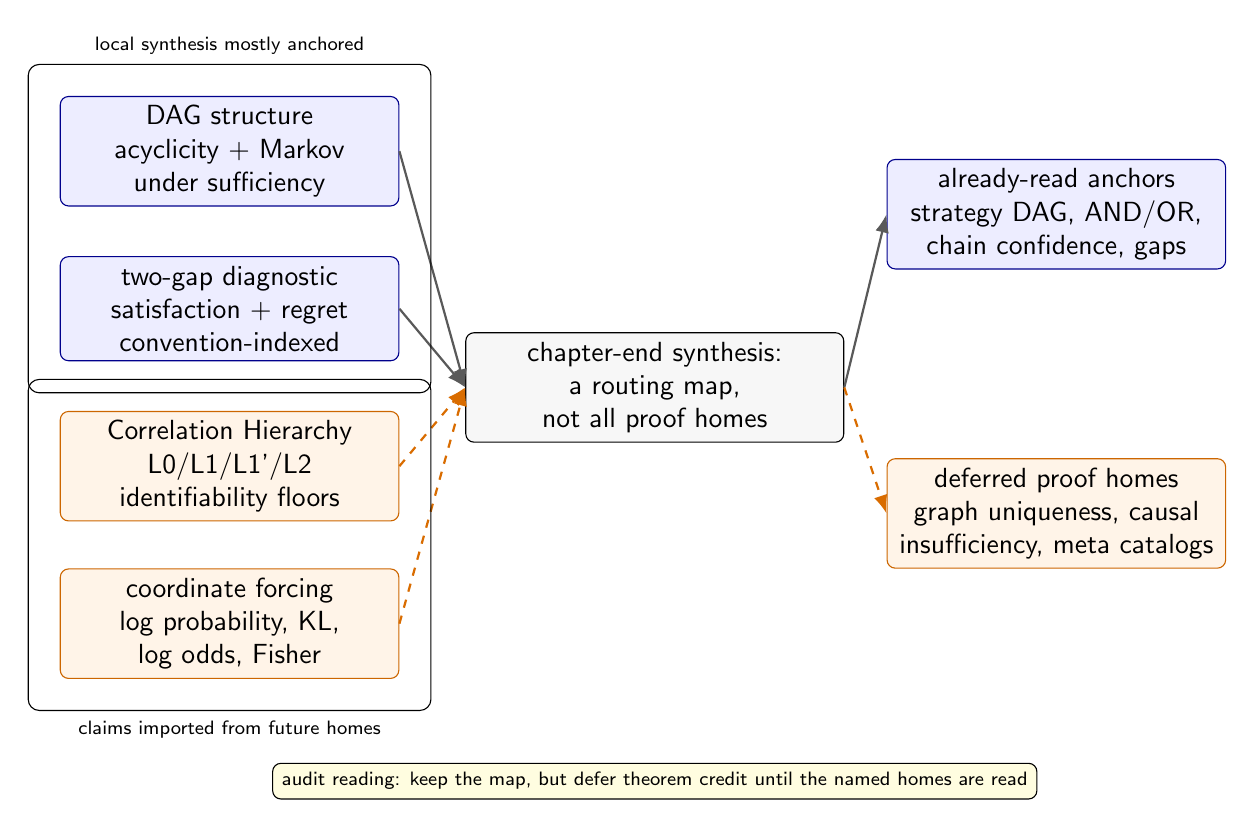
\begin{tikzpicture}[
  font=\sffamily,
  block/.style={draw, rounded corners=3pt, align=center, minimum width=43mm, minimum height=12mm, fill=white},
  local/.style={block, fill=blue!7, draw=blue!55!black},
  future/.style={block, fill=orange!9, draw=orange!80!black},
  note/.style={align=center, font=\sffamily\scriptsize},
  arrow/.style={-Latex, thick, draw=black!65},
  defer/.style={-Latex, thick, dashed, draw=orange!85!black}
]

\node[local] (dag) at (0,3)
  {DAG structure\\acyclicity + Markov\\under sufficiency};
\node[local] (gaps) at (0,1)
  {two-gap diagnostic\\satisfaction + regret\\convention-indexed};
\node[future] (corr) at (0,-1)
  {Correlation Hierarchy\\L0/L1/L1'/L2\\identifiability floors};
\node[future] (coord) at (0,-3)
  {coordinate forcing\\log probability, KL,\\log odds, Fisher};

\node[block, fill=gray!6, minimum width=48mm] (chapter) at (5.4,0)
  {chapter-end synthesis:\\a routing map,\\not all proof homes};

\node[local] (done) at (10.5,2.2)
  {already-read anchors\\strategy DAG, AND/OR,\\chain confidence, gaps};
\node[future] (later) at (10.5,-1.6)
  {deferred proof homes\\graph uniqueness, causal\\insufficiency, meta catalogs};

\draw[arrow] (dag.east) -- (chapter.west);
\draw[arrow] (gaps.east) -- (chapter.west);
\draw[defer] (corr.east) -- (chapter.west);
\draw[defer] (coord.east) -- (chapter.west);

\draw[arrow] (chapter.east) -- (done.west);
\draw[defer] (chapter.east) -- (later.west);

\node[note, fill=yellow!12, draw, rounded corners=3pt, minimum width=86mm] at (5.4,-5.0)
  {audit reading: keep the map, but defer theorem credit until the named homes are read};

\node[draw, rounded corners=4pt, fit=(dag)(gaps), inner sep=4mm,
  label={[note]above:local synthesis mostly anchored}] {};
\node[draw, rounded corners=4pt, fit=(corr)(coord), inner sep=4mm,
  label={[note]below:claims imported from future homes}] {};

\end{tikzpicture}
\end{document}
